\documentclass[12pt]{article}
\usepackage[utf8]{inputenc}
\usepackage[T1]{fontenc}
\usepackage{graphicx}
\usepackage{hyperref}

\title{Cahier des Charges Projet MLOps}
\author{}
\date{}

\begin{document}

\maketitle

\section{Contexte et Objectifs}

Ce projet s’inscrit dans une démarche d’optimisation de l’organisation des forces de l’ordre de la ville de Chicago, notamment en étant capable de prédire des pics de criminalité. Pour une grande ville comme Chicago, il est pertinent de pouvoir prévenir si cela est possible l’apparition de crimes et de surcroît renforcer les équipes lorsque cela est nécessaire, ce qui améliore les délais d’intervention.

La ville de Chicago souhaite la mise en place d’une application évolutive et qui analyse et prédit les données en temps réel. Cette API lui permettra d’améliorer son organisation, sa prise de décision et à optimiser ses opérations et ses ressources humaines. Pour la réalisation de cette API, la ville met à disposition des ressources, c'est-à-dire un dataset contenant le rapport des crimes survenus dans la ville depuis 2001. Ce dataset est mis à jour régulièrement.

Les utilisateurs principaux sont tous utilisateurs finaux ayant les droits d’accès à l’application (Forces de l’ordre, administration etc.)

L’administration et la maintenance de l’application sera effectuée par l’équipe technique en charge de la ville de Chicago. Ceux-ci auront la responsabilité de maintenir à jour, déployer, surveiller les performances et améliorer si besoin l’API pour assurer son fonctionnement optimal.

L'API sera hébergée sur une infrastructure cloud, assurant ainsi flexibilité, haute disponibilité et adaptabilité en fonction de la demande. Cette configuration cloud favorise également une harmonisation aisée avec les systèmes et services déjà en place.

Pour une interaction directe, les utilisateurs finaux pourront accéder à l'API via une plateforme web dotée d'une interface utilisateur conviviale. Par ailleurs, pour une intégration plus poussée et une automatisation avancée, les développeurs et les administrateurs bénéficieront d'un accès direct à l’API, permettant une synergie fluide avec d'autres outils et processus existants.

Pour faire face à cette problématique, nous envisageons la mise en place d'une API spécifiquement 
conçue pour la prédiction des événements criminels. En exploitant les technologies de pointe et en l'hébergeant sur une infrastructure cloud, nous assurons une solution flexible et hautement disponible. Cette API offrira la capacité de réaliser des prédictions en temps réel en se basant sur des données existantes.

\section{Modèle}

\subsection{Collecte des données}

La collecte des données sur les crimes est organisée de manière, où chaque incident est classifié non seulement par région, mais aussi chronologiquement par mois. Cette approche transforme le nombre de crimes en une série temporelle, permettant ainsi une analyse des tendances et des modèles dans le temps.

\subsection{Types de crime}

\begin{itemize}
    \item DECEPTIVE PRACTICE
    \item OTHER OFFENSE
    \item THEFT
    \item ...
\end{itemize}

\subsection{Type de région}

\begin{itemize}
    \item Rogers Park
    \item West Ridge
    \item Uptown
    \item ...
\end{itemize}

\subsection{Modélisation et Prédiction}

Pour anticiper et comprendre l'évolution future de ces tendances criminelles, nous avons intégré l'utilisation d'un outil analytique et de prédiction des séries temporelles Prophet, accessible via PyPI.
Le package Prophet  intègre et traite les variations saisonnières ainsi que les impacts des jours fériés, ce qui rend ses prédictions particulièrement robustes et fiables. Ces prédictions sont essentielles pour la mise en place d'une stratégie de planification efficace et pour une allocation optimale des ressources dans le cadre de la lutte contre la criminalité.

\subsection{Code et Implémentation}

Le cœur de notre modèle est incarné par la classe \texttt{ChicagoCrimePredictor}, structurée comme suit : \texttt{ChicagoCrimePredictor(months\_pred=12, data\_dir=DATA\_DIR)}.

Cette classe est conçue pour être flexible et adaptative, avec deux arguments principaux lors de l'initialisation :

\begin{itemize}
	\item \texttt{months\_pred}: Cet argument détermine la période de prédiction, permettant aux utilisateurs de spécifier le nombre de mois pour lesquels ils souhaitent obtenir des prévisions.
	\item \texttt{data\_dir}: Il s'agit du répertoire contenant les données brutes, permettant au modèle d'accéder et de traiter l'ensemble des informations nécessaires.
\end{itemize}

\subsection{Exemple d'application}

Dans le cas d'étude présenté, le modèle est entraîné sur les données collectées depuis l'année 2001 jusqu'en décembre 2022. À partir de ces données, des prédictions sont générées pour une durée d'un an, couvrant la période de janvier 2023 à décembre 2023. Cette approche permet non seulement de comprendre les tendances passées mais aussi d'anticiper avec une certaine précision les évolutions futures dans le domaine de la criminalité.

\paragraph{Focus sur la Criminalité dans la Région d'Austin:}
Pour cette étude, nous avons choisi de concentrer nos efforts sur la prédiction des crimes de type “ASSAULT” dans la région spécifique d'Austin. Cette focalisation est guidée par l'importance croissante de comprendre et de prévenir les actes de violence dans cette zone. Notre modèle, grâce à la méthode \texttt{return\_data}, est configurable et peut être adapté selon différents paramètres, notamment:

\begin{itemize}
	\item \texttt{type\_incident} : Permet de spécifier le type de crime à analyser, dans notre cas “ASSAULT”.
	\item \texttt{community\_area} : Cible une région spécifique pour la prédiction, ici la région d'Austin.
\end{itemize}



\subsection{Métriques d’évaluation}

\subsubsection{Mean Absolute Error (MAE)}

\textbf{Formule:} 
\[ MAE = \frac{1}{n} \sum_{i=1}^{n} \left| y_i - \hat{y}_i \right| \]

\textbf{Description :} Le MAE mesure la différence moyenne entre les valeurs observées (réelles) et les valeurs prédites par le modèle. Pour le calculer, on prend la différence absolue (sans tenir compte du signe) entre chaque paire de valeurs observée et prédite, et ensuite on calcule la moyenne de ces différences.

\textbf{Interprétation :} Un MAE plus petit indique une meilleure performance du modèle. C'est une mesure facile à comprendre car elle est exprimée dans les mêmes unités que les données observées. Par contre, comme elle utilise la valeur absolue, elle ne tient pas compte de la direction des erreurs (sous-estimation ou sur-estimation).

\subsubsection{Root Mean Squared Error (RMSE)}

\textbf{Formule:} 
\[ RMSE = \sqrt{\frac{1}{n} \sum_{i=1}^{n} (y_i - \hat{y}_i)^2} \]

\textbf{Description :} Le RMSE est similaire au MAE mais donne plus de poids aux erreurs plus grandes. On calcule d'abord la différence entre chaque valeur observée et prédite, on élève ces différences au carré, puis on en calcule la moyenne. Finalement, on prend la racine carrée de cette moyenne.

\textbf{Interprétation :} Un RMSE plus faible signifie une meilleure précision du modèle. Le RMSE est plus sensible aux erreurs importantes, ce qui peut être un avantage dans certains contextes où ces erreurs sont plus problématiques. Comme le MAE, le RMSE est exprimé dans les mêmes unités que les valeurs observées.

\subsubsection{R2 (Coefficient de détermination)}

\textbf{Formule:} 
\[ R^2 = 1 - \frac{\sum_{i=1}^{n} (y_i - \hat{y}_i)^2}{\sum_{i=1}^{n} (y_i - \bar{y})^2} \]

\textbf{Description :} Le R2 mesure la proportion de la variance des valeurs observées qui est expliquée par le modèle. Il est calculé en comparant la variance des erreurs du modèle avec la variance totale des valeurs observées.

\textbf{Interprétation :} Un R2 proche de 1 indique que le modèle explique une grande partie de la variance des données, tandis qu'un R2 proche de 0 indique que le modèle n'explique pas bien la variance des données. Le R2 est une mesure utile pour comparer différents modèles entre eux, mais il ne doit pas être le seul critère de jugement, surtout si les données ne suivent pas une distribution normale ou si le modèle est complexe.


\subsection{Résultats d’évaluation}

\begin{figure}[htbp]
	\centering
	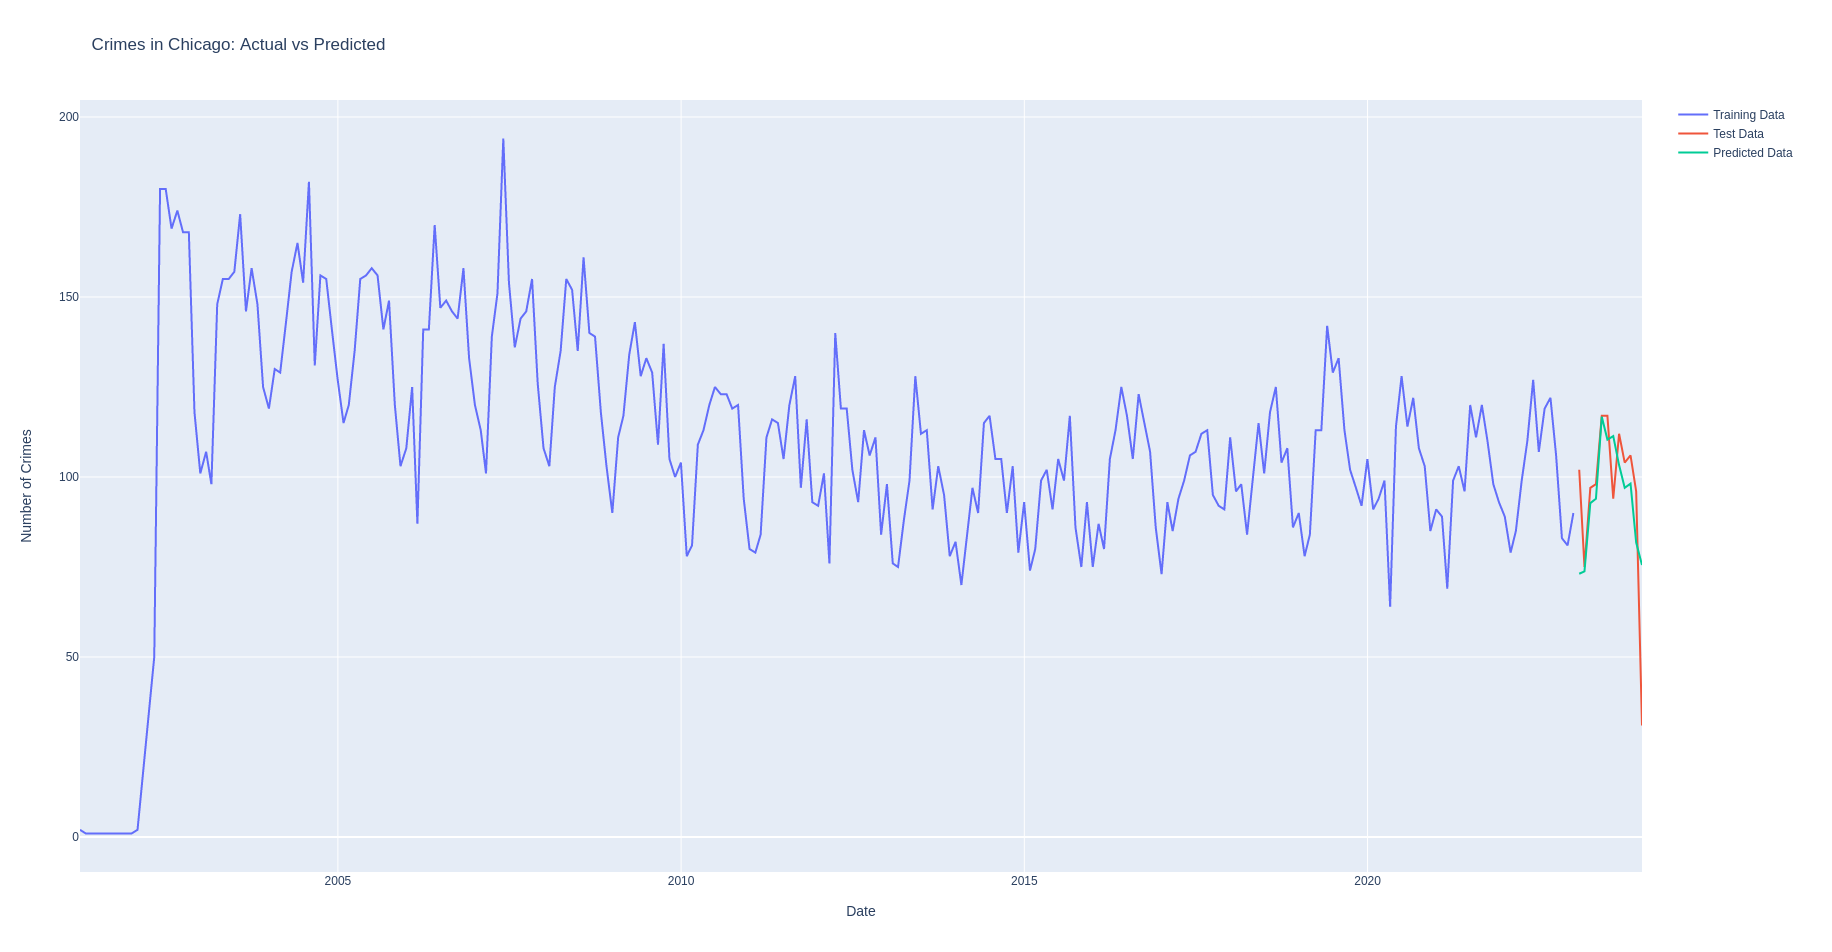
\includegraphics[width=0.7\textwidth]{figure_Assault_Austin.png}
	\caption{Résultats de l'évaluation pour les crimes de type ASSAULT dans la région d'Austin.}
	\label{fig:assault_austin}
\end{figure}

\begin{table}[htbp]
	\centering
	\caption{Métriques du modèle pour les crimes de type ASSAULT dans la région d'Austin}
	\begin{tabular}{|l|c|}
		\hline
		Métrique & Valeur \\
		\hline
		Mean Absolute Error (MAE) & 12.06 \\
		Root Mean Squared Error (RMSE) & 17.28 \\
		R² & 0.4 \\
		\hline
	\end{tabular}
	\label{tab:metrics_assault_austin}
\end{table}
Une base de données SQLite a été créée, permettant ainsi l'enregistrement des métriques pour chaque exécution.
\begin{figure}[htbp]
	\centering
	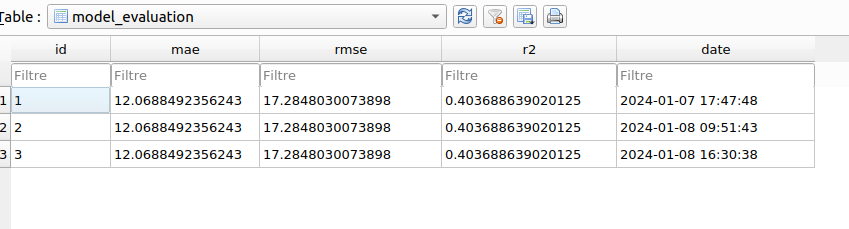
\includegraphics[width=0.7\textwidth]{Capture_Sqlite.png}
	\caption{Résultats de l'évaluation : capture base de donnée Sqlite}
	\label{fig:assault_austin}
\end{figure}



\section{API}

\section{Testing \& Monitoring}

\section{Schéma d’implémentation}

\end{document}
